%%%%%%%%%%%%%%%%%%%%%%%%%%%%%%%%%%%%%%%%%%%%%%%%%%%%%%%%%%%%%%
\subsection{Детектирование ШПС от одного источника}
Рассмотрим простой случай - поиск гармонического сигнала на фоне АБГШ (интерференция отсутствует).
\label{l:sec3_lpc}

Пусть входной сигнал после снятия кода может быть представлен в виде:
\begin{center}
\begin{equation}
	\label{eq:lpc_signal_model1}
	x(k) = AC(k)D(k)\cos(\omega k) + n(k)
\end{equation}
\end{center}
где: ${A}$ - мощность сигнала, ${C}$ - ПСП, ${D}$ - данные, а ${\omega_{c}}$ - частота несущей сигнала.
Детектирование сигнала происходит в пределах одного бита данных. В этом случае ${D(k)}$
принимается как константа. Повторная модуляция сигнала приводит к выражению ${C(k)C(k)=1}$.
Таким образом \ref{eq:lpc_signal_model1} можно записать как:
\begin{center}
\begin{equation}
	\label{eq:lpc_signal_model2}
	x(k)= A \cos{(\omega k)} + z(k)
\end{equation}
\end{center}

Поскольку ${n(k)}$ - случайный процесс, то ${z(k) = n(k)C(k)}$ также является
случайным процессом. Определим числовые характеристики ${z(k)}$.
В виду того что ${C(k)}$ и ${n(k)}$ - независимы, а ${D[C] = 1}$,можно записать:

\begin{center}
\begin{equation}
	%\label{}
	D[z(k)] = D[nC] = D[n] = \sigma ^2
\end{equation}
\end{center}
Таким образом ${z(k)}$ - АБГШ помеха.

Для уравнения \ref{eq:lpc_gps_1}, необходимо вычислить ковариации для 3 точек
${r_{xx}(0)}$, ${r_{xx}(1)}$, ${r_{xx}(2)}$, используя выражение \ref{eq:lpc_rxx_estimation}.
Оценка частоты сигнала может быть получена из выражения \ref{eq:lpc_poles_freq}, а его
мощность из \ref{eq:lpc_power_cos}.

Можно построить график оценки СПМ для смещения,
содержащего максимальный спектральный пик - гармоническую компоненту
с наивысшей энергией - рисунок \ref{pic:lpc_psd_1} и график состоящий из максимальных спектральных пиков для каждой фазы
ПСП - рисунок \ref{pic:lpc_1sat_energy}.

\begin{figure}[H]
	\center\scalebox{1}{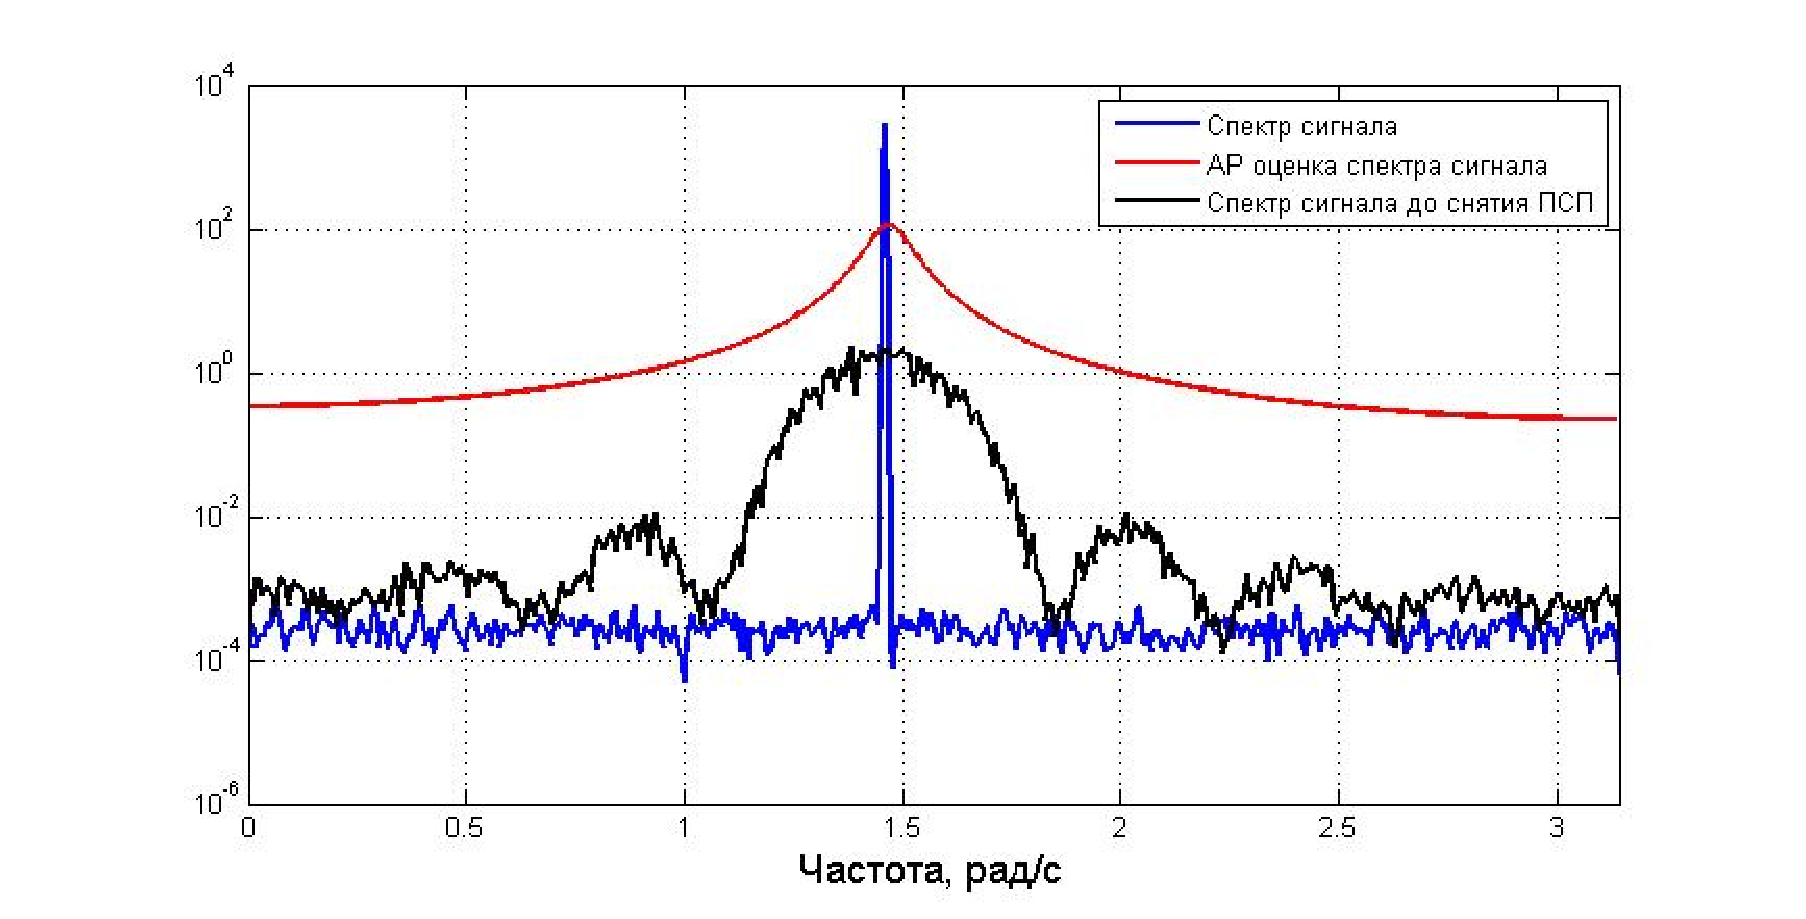
\includegraphics[width=1\linewidth]{lpc_1sat.eps}}
	\caption{Оценка СПМ сигнала модулированного ПСП}
	\label{pic:lpc_psd_1}
\end{figure}
\begin{figure}[H]
	\center\scalebox{1}{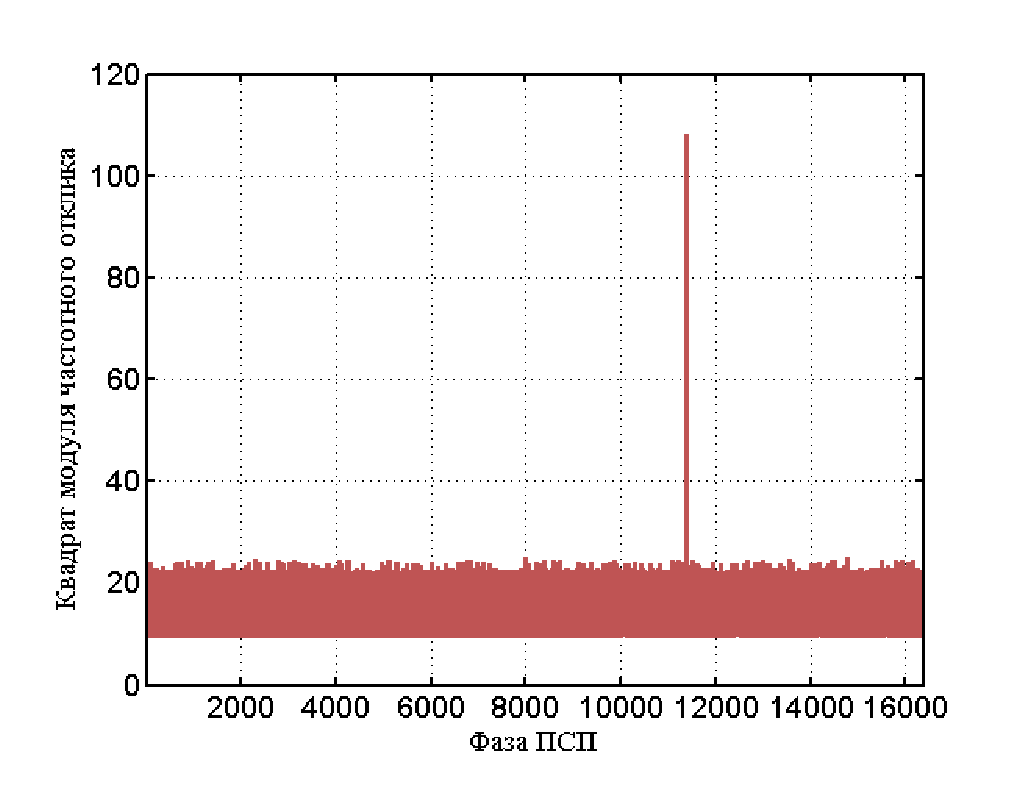
\includegraphics[width=1\linewidth]{lpc_1sat_energy.eps}}
	\caption{Квадраты частотного отклика для всех возможных фаз ПСП}
	\label{pic:lpc_1sat_energy}
\end{figure}



%%%%%%%%%%%%%%%%%%%%%%%%%%%%%%%%%%%%%%%%%%%%%%%%%%%%%%%%%%%%%%
\subsubsection{Влияние интерференции на точность детектирования с помощью АР модели}
Шум, отличный АБГШ будет смещать оценку частоты. На рисунке \ref{pic:lpc_2sat_psd} показано
смещение для интерференционной помехи от еще одного источника сигнала, модулированной ПСП того же семейства.
Данная помеха не является белой и оценка АР-методом по предложенному алгоритму не даст надежной оценки частоты сигнала.

\begin{figure}[H]
	\center\scalebox{1}{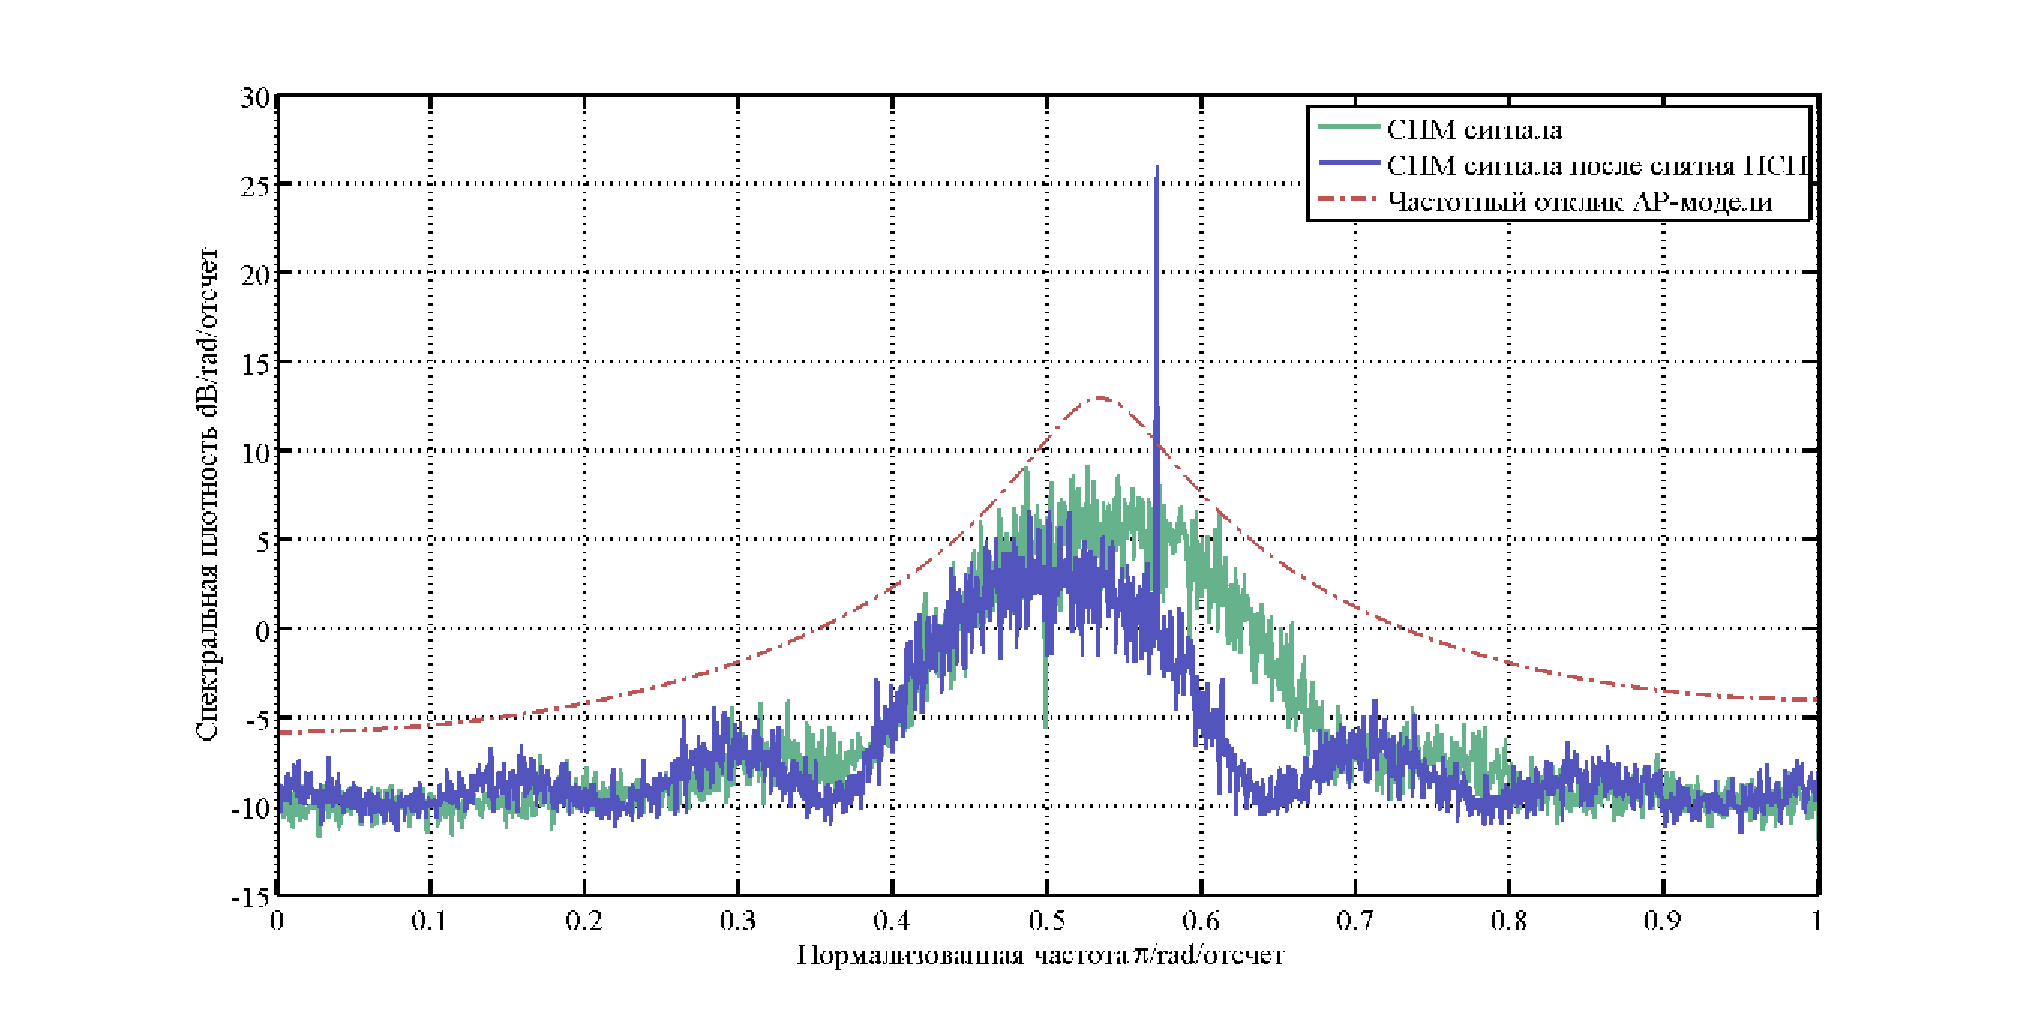
\includegraphics[width=1\linewidth]{lpc_2sat_psd.eps}}
	\caption{СПМ для сигнала с интерференционной помехой}
	\label{pic:lpc_2sat_psd}
\end{figure}

\subsection*{Выводы}
\label{ssec:sec3_lpc_conclusion}

В данном разделе предложен алгоритм детектирования ШПС на основе АР-модели принимаемого сигнала.
Разработанный алгоритм позволяет производить оценку частоты гармонического сигнала без использования прямого
перебора как это делается в большинстве современных алгоритмов. Например, алгоритм Delay and Multiply Approach (DMA) предложенный в 
\cite{lin_dma, tsui} позволяет производить поиск только по смещению ПСП, но он не дает возможности прямой оценки частоты.
Для оценки частоты и принятия решения о наличии сигнала в алгоритме DMA необходимо использовать стандартный коррелятор.

К недостаткам данного подхода можно отнести: 
\begin{enumerate}
	\item Сравнительно высокие вычислительные затраты. Предложенный алгоритм требует поиск гармонической
		компоненты, а так же обращения теплицевой матрицы для каждого смещения ПСП.
	\item Сильная чувствительность по отношению к интерференционным помехам: наличие
		''окрашенного'' шума приводит к значительному смещению получаемых
		оценок частоты и мощности гармонического сигнала.
\end{enumerate}

%%%%%%%%%%%%%%%%%%5
% OLD
%%%%%%%%%%%%%%%%%%5

%\subsection*{\textcolor{red}{Старый текст для переноса!!!!!!!!!}}
%
%\subsubsection{Влияние теплового шума на точность детектирования с помощью АР модели}
%%Для применения АР метода является очень существенным знать модель шумовой компоненты из ${n(t)}$ из выражения
%%		r_{xx}(2)
%%\ref{eq:lpc_signal}. Зная АКФ ${n(t)}$, можно получить несмещенную оценки ${\omega_c}$.
%
%\subsubsection{Детектирование ШПС от одного источника}
%
%
%Но любой шум, отличный АБГШ будет смещать оценку частоты. На рисунке \ref{pic:lpc_1sat_interference}
%представлен график смещения оценки в зависимости от мощности второго луча сигнала, модулированного
%той же ПСП.
%
%\begin{figure}[H]
%	\center\scalebox{1}{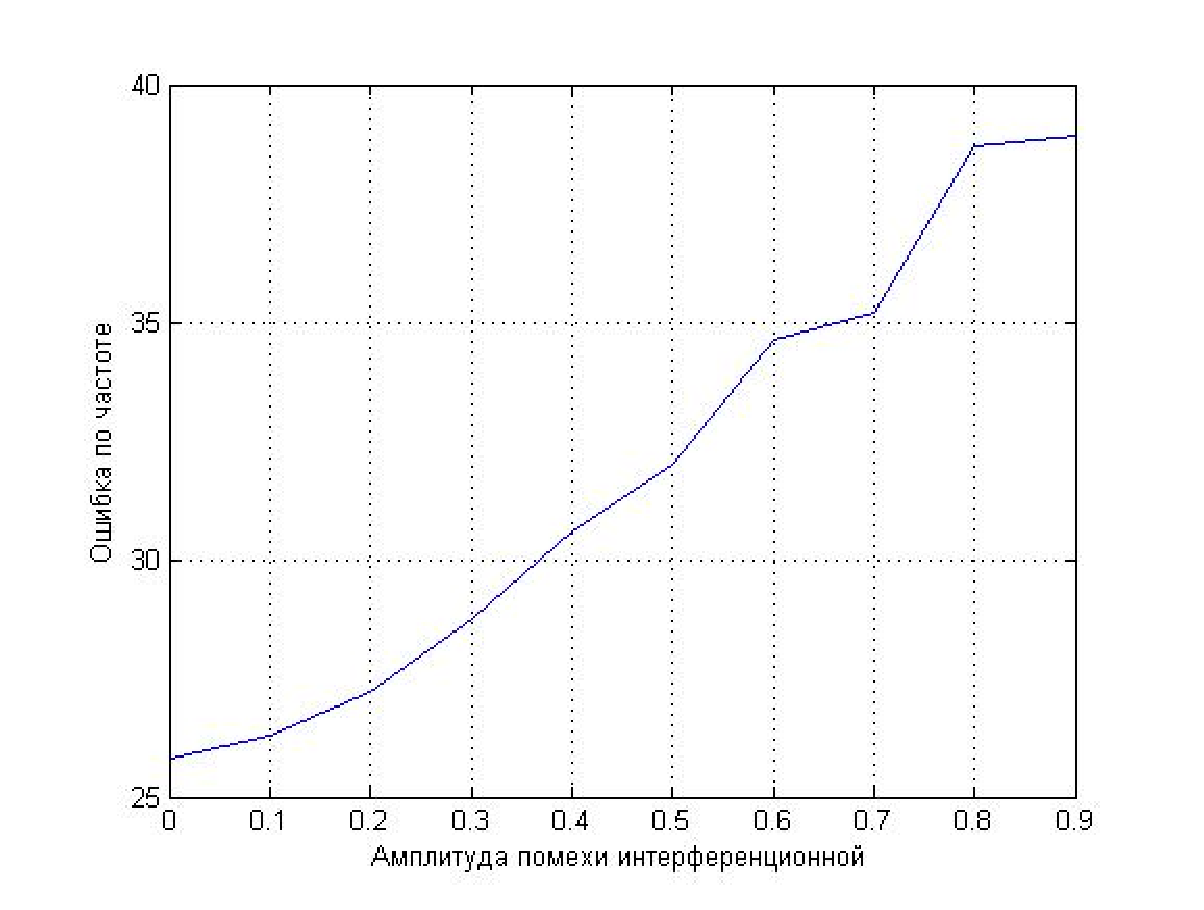
\includegraphics[width=1\linewidth]{lpc_interference.eps}}
%	\caption{Зависимость ошибки оценки пика от энергии интерференционной помехи}
%	\label{pic:lpc_1sat_interference}
%\end{figure}
%
%%%%%%%%%%%%%%%%%%%%%%%%%%%%%%%%%%%%%%%%%%%%%%%%
%\subsubsection{Детектирование ШПС с коррекцией шума}
%
%Для детектирования слабых сигналов, необходимо знать природу шума. Тепловой шум является одинаковым для всех источников,
%таким образом его можно получить от других приемников или рассчитать в процессе детектирования. 
%
%Для некоторых существующих систем на основе сигналов, модулированных ПСП, можно использовать приемники находящиеся рядом,
%ввиду, что приемников данного сигнала достаточно большое количество. В качестве примера можно взять сигнал Navstar GPS
%для приемников. Достаточно большое количество приемников GPS, захвативших сигнал, находится вблизи приемника, который
%только начинает процедуру детектирования сигнала. По такой схеме работает система AGPS (Assistance GPS). Так же по данной
%схеме работает система, разработанная в процессе исследований. Эта система отражена в заявке на изобретение
%\cite{patent_my}.
%
%\begin{center}
%\begin{equation}
%	\label{eq:lpc_a_estimation}
%	\left[ \begin{array}{c}
%		\hat{a}_1 \\
%		\hat{a}_2
%	\end{array} \right]
%		=
%		\left(
%			\left[ \begin{array}{cc}
%				r_{xx}(0) & r_{xx}(1) \\
%				r_{xx}(1) & r_{xx}(0)
%			\end{array} \right] -
%			\left[ \begin{array}{cc}
%				n_{xx}(0) & n_{xx}(1) \\
%				n_{xx}(1) & n_{xx}(0)
%			\end{array} \right] 
%		\right)
%		\left[ \begin{array}{c}
%			r_{xx}(1) \\
%			r_{xx}(2)
%		\end{array} \right]
%		=
%		R_x^{-1}r_{xx1}
%\end{equation}
%\end{center}
%
%%%%%%%%%%%%%%%%%%%%%%%%%%%%%%%%%%%%%%%%%%%%%%%%
%\subsubsection{Детектирование ШПС с коррекцией шума}
%Точность АР метода напрямую зависит от точности оценки АКФ гармонического сигнала. Основным способом повышения точности оценки
%АКФ является увеличение размера выборки, что в случае модулированного сигнала может быть затруднительным. В данной работе
%предлагается алгоритм оценки АКФ гармонического сигнала, не требующий увеличения длины или накопления сигнала.
%Повышение точности достигается за счет того, что АКФ гармонического сигнала представляет собой гармонический сигнал той же частоты.
%Пусть входной сигнал после снятия кода может быть представлен в виде:
%
%\begin{center}
%\begin{equation}
%	%\label{eq:lpc_gps_1}
%	x(k)=A \cos{(\omega_k)} + n(k)
%\end{equation}
%\end{center}
%
%где ${n(k)}$ - АБГШ помеха. Тогда оценка АКФ сигнала ${x(k)}$:
%
%
%\begin{center}
%\begin{equation}
%	%\label{eq:lpc_gps_1}
%	r_1 = F^{-1}[Fx \cdot Fx]
%\end{equation}
%\end{center}
%
%где ${F}$ - матрица преобразования Фурье, ${F^{-1}}$ - обратная матрица преобразования Фурье, ${x}$ - вектор входного сигнала,
%демодулированного ПСП, а (${\cdot{}}$) - знак означает поэлементное перемножение векторов.
%
%\begin{center}
%\begin{equation}
%	%\label{eq:lpc_gps_1}
%	r_1 = F^{-1} \left[ F\left[F^{-1}\left[Fx \cdot Fx\right]\right] \cdot F\left[F^{-1}\left[Fx \cdot Fx\right]\right] \right]
%\end{equation}
%\end{center}
%
%%Специфичной для детектирования ШПС является необходимость определения точной фазы ПСП
%%для работы с сигналом. Так же при обработке ШПС от нескольких источников с разными ПСП необходимо учитывать,
%%что оценка спектра будет смещенной и требуется его корректировка. Следует учитывать, что после демодуляции
%%с синхронизированной копией ПСП получается гармоничнская компонента и шум. Подробнее компоненты шума были
%%рассмотрены в \ref{l:noise_model}. Преобразуем выражение \ref{eq:gps_signal_modulated}: амплитуду гармонического
%%сигнала возьмем ${\sqrt{2A} = 1}$, ${D_k(t)}$ примем за 1, учитывая, что мы детектируем сигнал в пределах одного
%%чипа:
%%\begin{center}
%%\begin{equation}
%%	%\label{eq:lpc_signal}
%%	s(t) = \cos(\omega_{c}t) + n(t)
%%\end{equation}
%%\end{center}
%
%\newpage
